\documentclass[onecolumn]{aastex63}
\usepackage{natbib}
%\definecolor{orcidlogocol}{HTML}{A6CE39}
\bibliographystyle{aasjournal}

\begin{document}

\title{COLLISION RATES OF PLANETESIMALS NEAR MEAN-MOTION RESONANCES}

\author{Spencer C. Wallace}
\affiliation{Astronomy Department, University of Washington, Seattle, WA 98195}

\author{Aaron C. Boley}
\affiliation{Department of Physics and Astronomy, University of British Columbia, Vancouver BC, Canada}

\author{Thomas R. Quinn}
\affiliation{Astronomy Department, University of Washington, Seattle, WA 98195}

\begin{abstract}
In circumstellar disks, collisional grinding of planetesimals produces second-generation dust, which can be observed through thermal 
emission. While it remains unclear when second-generation dust first becomes a major component of the total dust content, the presence of 
such dust and potentially the substructure within it can be used to explore a disk's physical conditions. A perturbing planet has been shown to 
produce nonaxisymmetric structures, as well as gaps in disks, regardless of the origin of the dust. However, small grains will have very 
different dynamics compared with planetesimals when in the presence of gas, and as such, the collisional evolution of planetesimals could 
create dusty disk structures that would not exist otherwise. In particular, mean motion resonances (MMRs) are extremely nonlinear and could 
drive disk morphologies. We use a direct N-body model to track collision rates in a planetesimal disk under the gravitational influence of an 
external Jupiter-sized planet. We show that a perturbing planet can produce significant variations in the collision rate of planetesimals near the 
MMRs and we explore how the mass and eccentricity of the perturbing planet alters this structure. Finally, we use the CASA image simulator to 
predict what the dust emission sturcture should look like with ALMA and the NG-VLA. Although the dust structure produced by MMRs cannot 
be used to directly measure the properties of the perturbing planet, we show that it can be used to place constraints on its mass and 
eccentricity.
\end{abstract}

\section{Introduction} \label{sec:intro}

Recent observations of circumstellar disks by ALMA have revealed a rich variety of substructure in the millimeter wavelength
contiunuum emission. Features such as gaps and asymmetries 
\citep{2015ApJ...808L...3A, 2016Sci...353.1519P, PhysRevLett.117.251101, 2016ApJ...820L..40A, 2016Natur.535..258C} in the 
emission provide diagnostics for the physical processes that drive the evolution of the disks. At these wavelengths, much of this light 
is produced by second-generation debris generated through collisional grinding of planetesimals
\citep[see][]{2008ARA&A..46..339W}. 

In some cases, these gap features are argued to be an indicator for the presence of a giant planet, either embedded in the disk 
\citep{2015MNRAS.453L..73D} or orbiting externally. An giant perturber can influence the structure of the dust emission in a number 
of ways. A misaligned giant planet can produce nonaxisymmetric features such as warps \citep{2001A&A...370..447A}. Highly 
eccentric perturbers can produce even more complicated structures through secular perturbations \citep{2014MNRAS.443.2541P, 
2015MNRAS.448.3679P}. Mean motion resonances (MMRs) have been shown to open gaps as well
\citep{2015ApJ...798...83N, 2016ApJ...818..159T, 2018ApJ...857....3T}.

The dynamics governing the motion of bodies near MMRs is extremely nonlinear, as is determining what the collision rates between 
planetesimals should look like in these regions. For a collection of bodies massive enough to experience the effects of gravitational 
focusing, a large eccentricity dispersion tends to reduce the probability of collision, while enhancements in surface density tends to 
increase it. Due to conservation of the Jacobi energy, MMRs simultaneously enhance the local eccentricity dispersion and also 
enhance the surface density adjacent to the resonance \citep{2000Icar..143...45R, 2017ApJ...850..103B}.

Because the second generation dust production is driven by the planetesimal collision rate, it is crucial to understand how the 
dynamics that drive collisions works. In particular, it is not obvious how to link the readily observable thermal emission from dust in 
protoplanetary disks to the presence of a perturbing giant planet. Due to its nonlinearity, this problem is best studied with N-body 
simulations. Unfortunately, collision detection in an N-body simulation is extremely computationally expensive. So far, studies of 
planetesimal dynamics near MMRs have involved either collisionless test particles \citep{2017ApJ...850..103B, 2016ApJ...818..159T, 
2018ApJ...857....3T} or severely limited integration times \citep{2000Icar..143...45R}.

To further elucidate this subject, we use the tree based N-body code {\sc ChaNGa}
\citep{2008IEEEpds...ChaNGa, 2015AphCom..2..1} to follow the collisional evolution of a planetesimal disk under the gravitational 
influence of a Jupiter sized body. Because particle positions are sorted into a tree structure, neighbor finding and collision detection 
can be done quickly and efficiently. This considerably relaxes the constraints on resolution and integration time. With this toolset, we 
explore the collision rate structure of the planetesimal disk in the vicinity of mean motion resonances. In particular, we would like to 
determine: 1. whether MMRs leave a detectable signature in the collisionally-generated dust. 2. If these signatures can be used to determine the orbital properties of the perturbing planet.

Also mention \citet{2020A&A...635A..10S}, looked at dust trapping in resonances with terrestrial SS planets. Also mention 
\citet{2020arXiv200408736G}, detection of a planetesimal collision around Fomalhut.

This work is organized in the following way: In section \ref{sec:dynamics}, we provide an overview of the relevant dynamics that drive 
the evolution of a planetesimal disk under the gravitational influence of an external perturber. We also highlight the shortcomings of secular theory in trying to predict the radial collision rate and motivate the need for N-body simulations with massive, collisional particles. In section \ref{sec:sims} we describe the N-body code that we use and detail the initial conditions that are used for two simulations: one in which the perturber is on a circular orbit and another in which the perturber is given a mildly eccentric orbit. Section \ref{sec:results} presents the results of the two simulations. Next, we generate dust emission maps in section \ref{sec:dust}, under the assumption that collisionally-generated dust will quickly couple with the gas and circularize, and show that radial structure is produced in the vicinity of the MMRs. Using the dust emission maps, section \ref{sec:fitting} explores the feasibility of measuring properties of the perturbing planet from the MMR features in the dust. We then conclude in section \ref{sec:discuss}. 

\section{Overview of Relavant Dynamics} \label{sec:dynamics}

\subsection{Collision Rates of Massive Bodies}

\subsection{Mean Motion Resonances}

\section{Simulations} \label{sec:sims}

\subsection{Numerical Methods}\label{sec:methods}

\subsection{Initial Conditions}\label{sec:ics}

\subsection{Time Stepping Scheme}\label{sec:timestep}

\section{Results} \label{sec:results}

\begin{figure*}
\begin{center}
    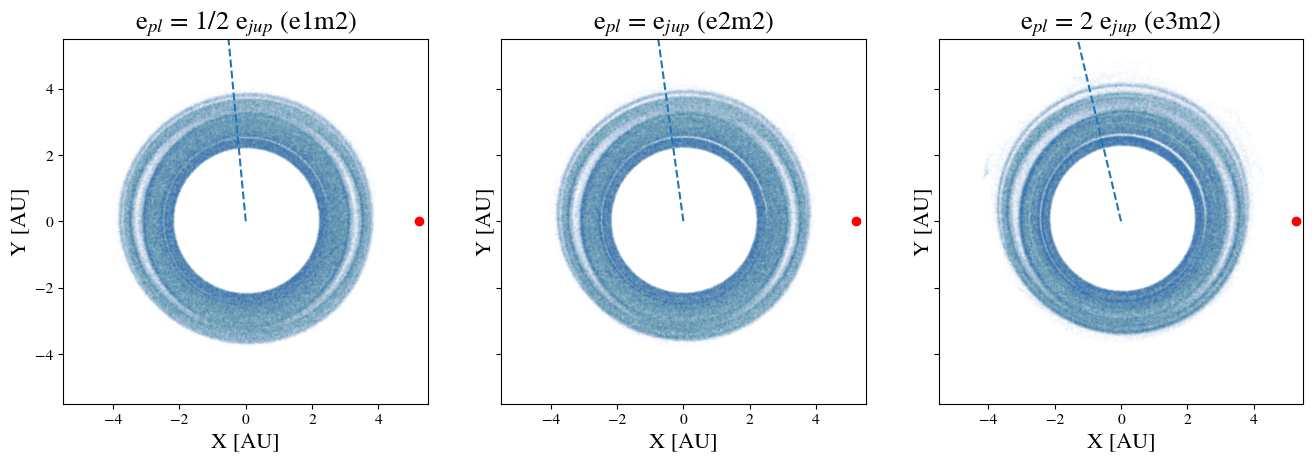
\includegraphics[width=\textwidth]{figures/xy.png}
    \caption{Non axisymmetric gaps and rings appear near MMRs. More features appear at higher eccentricities. Gap features
    at $\theta$ = 0 and $\theta = \pi$ follow the giant planet in its orbit.\label{fig:xy}}
\end{center}
\end{figure*}

\begin{figure}
\begin{center}
    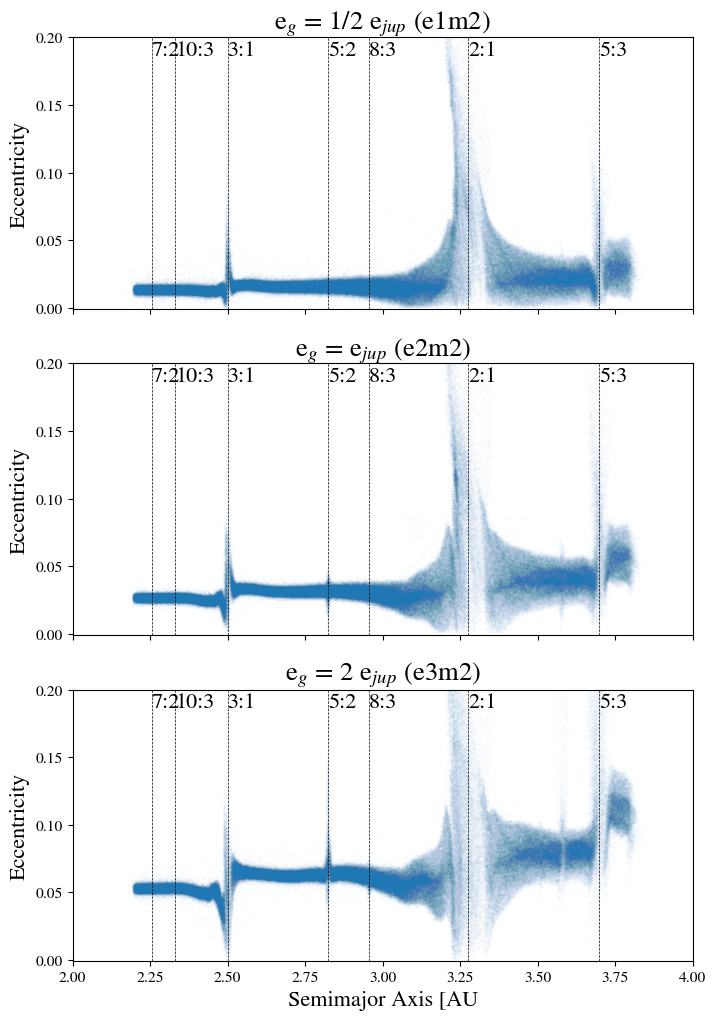
\includegraphics[width=0.5\textwidth]{figures/ae.png}
    \caption{The MMRs produce spikes in the a-e plane. Between resonances, the nonzero eccentricity is caused by secular
    forcing by the planet. At larger eccentricities, the higher order resonances become more prominent because of the steeper
    scaling with $e$.\label{fig:ae}}
\end{center}
\end{figure}

\begin{figure*}
\begin{center}
    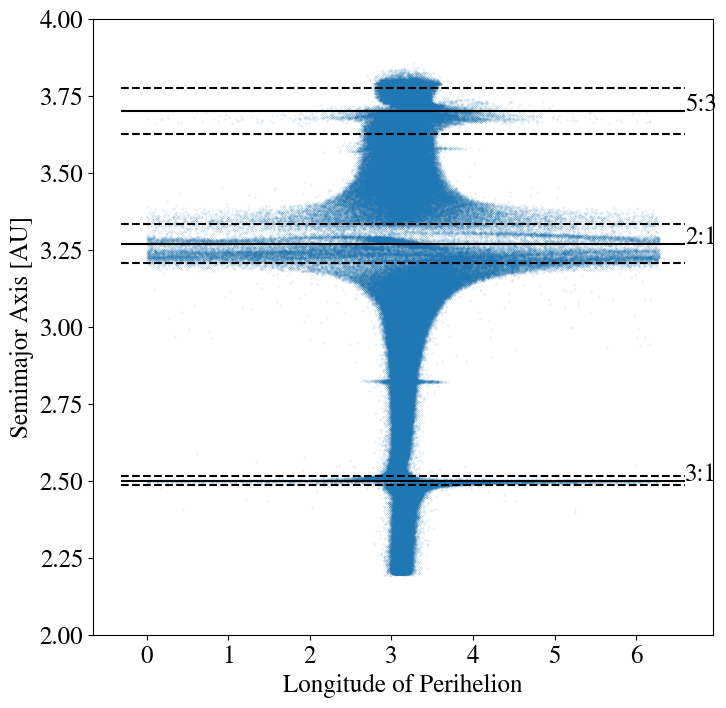
\includegraphics[width=\textwidth]{figures/long_ph.png}
    \caption{The MMRs also induce precession which overpowers the secular forcing. Inside of the resonances, orbits of
    planetesimals are effectively randomized.\label{fig:long_ph}}
\end{center}
\end{figure*}

\begin{figure}
\begin{center}
    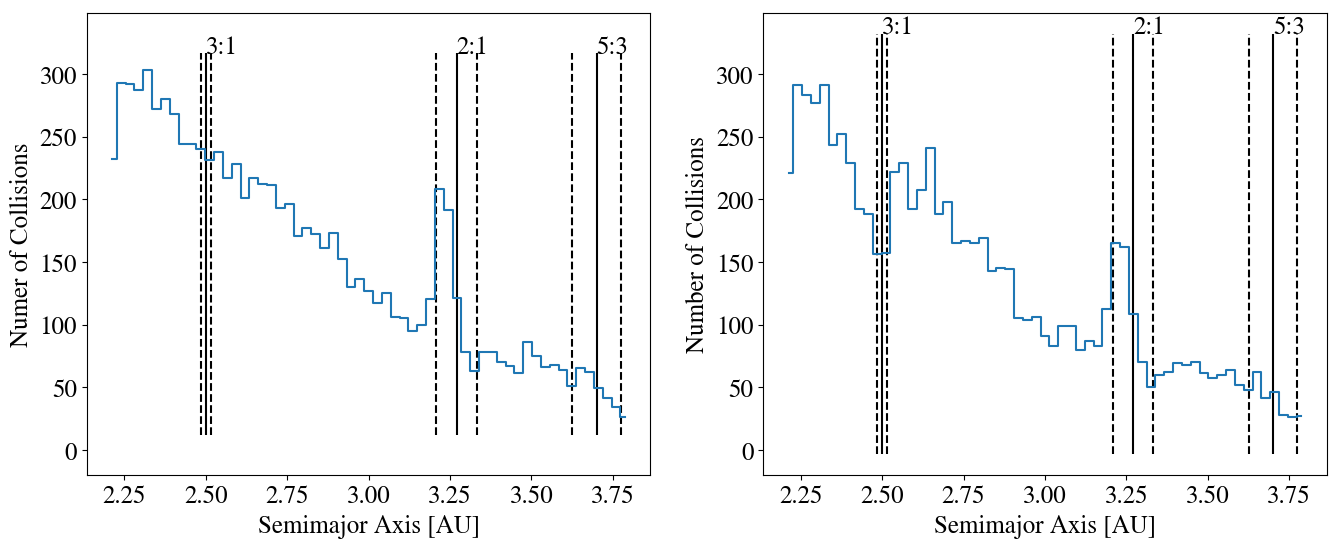
\includegraphics[width=0.5\textwidth]{figures/coll_hist_a.png}
    \caption{In semimajor axis space, prominent features appear near the 3:1 and 2:1 MMRs. Near the 3:1, the collision
    rate decreases, while it gets enhanced near the 2:1. This is because gravitational focusing is already suppressed
    near the 2:1. Additional heating by the resonance increases the encounter rate.\label{fig:coll_hist_a}}
\end{center}
\end{figure}

\begin{figure}
\begin{center}
    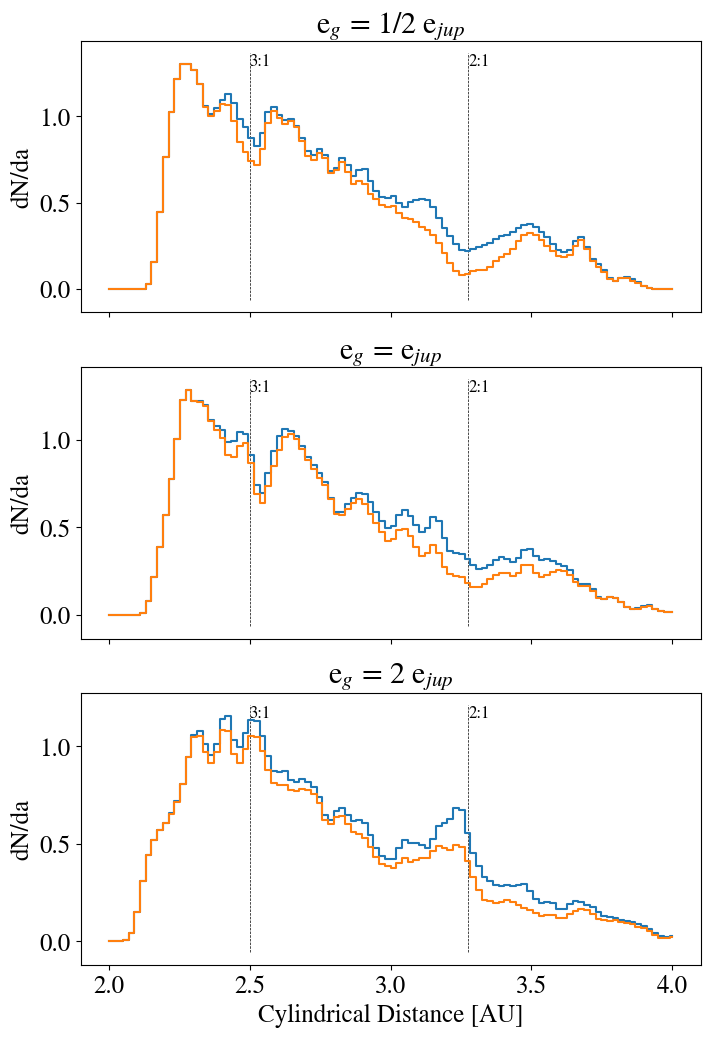
\includegraphics[width=0.5\textwidth]{figures/coll_hist_r.png}
    \caption{The features near resonance that appear in cylindrical distance space appear qualitatively different.
    The orange curve shows collisions with bodies inside the 2:1 and 3:1 MMR excluded. This does not qualitatively
    change any of the plots, and we infer that the features seen here are produced by bodies outside of resonance.
    Most interestingly,  the highest eccentricity planet simulation produces bumps, rather than dips near the 2:1 and
    3:1 MMR.\label{fig:coll_hist_r}}
\end{center}
\end{figure}

\begin{figure*}
    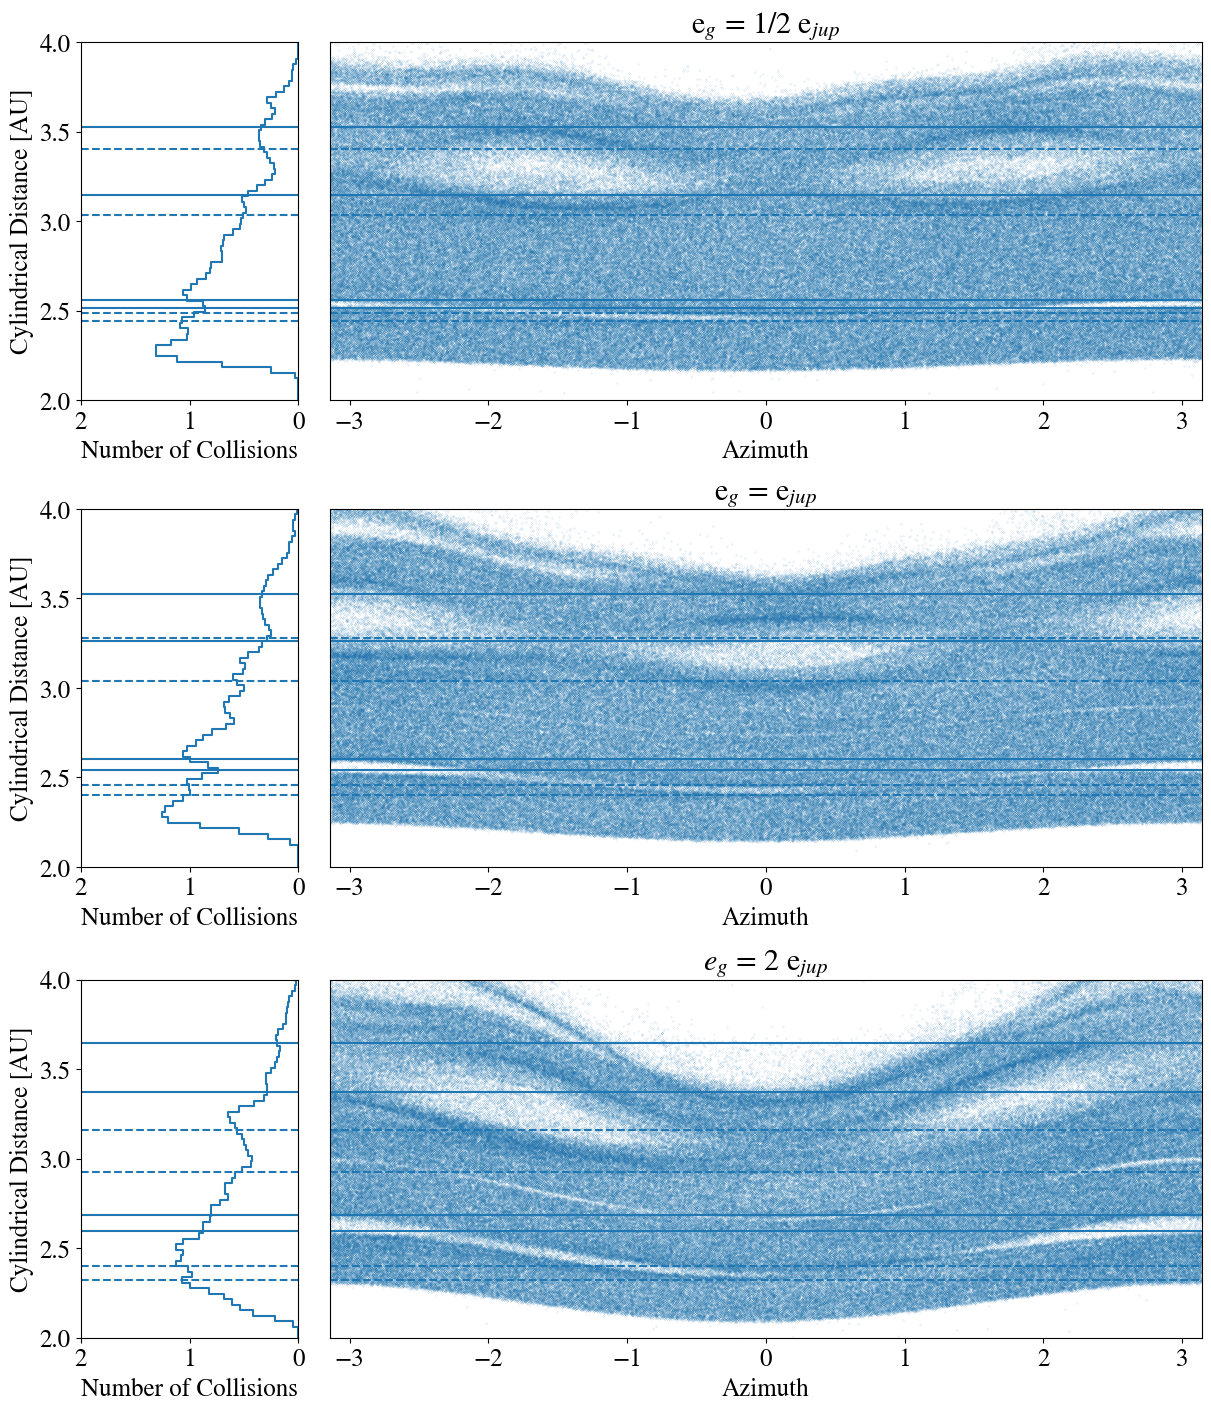
\includegraphics[width=\textwidth]{figures/coll_polar_e.png}
    \caption{The features in the previous figure appear to match with the pileups of bodies near the edges of the
    resonances. The dashed and solid lines show the perihelion and aphelion distances for bodies at the inner
    and outer edges of the 2:1 and 3:1 resonances. The dip vs bump features seen in the previous figure appear
    to depend on whether the aphelia of bodies at the inner edge and perihelia of bodies at the outer edge of a
    resonance cross. When this does not occur, a cavity persists at the center of the resonance, which reduces the
    collision rate in that region. When the two distances overlap, bodies from both edges of the resonance spend some
    time in the middle, producing a bump in the collision rate.\label{fig:coll_polar_e}}
\end{figure*}

\begin{figure*}
    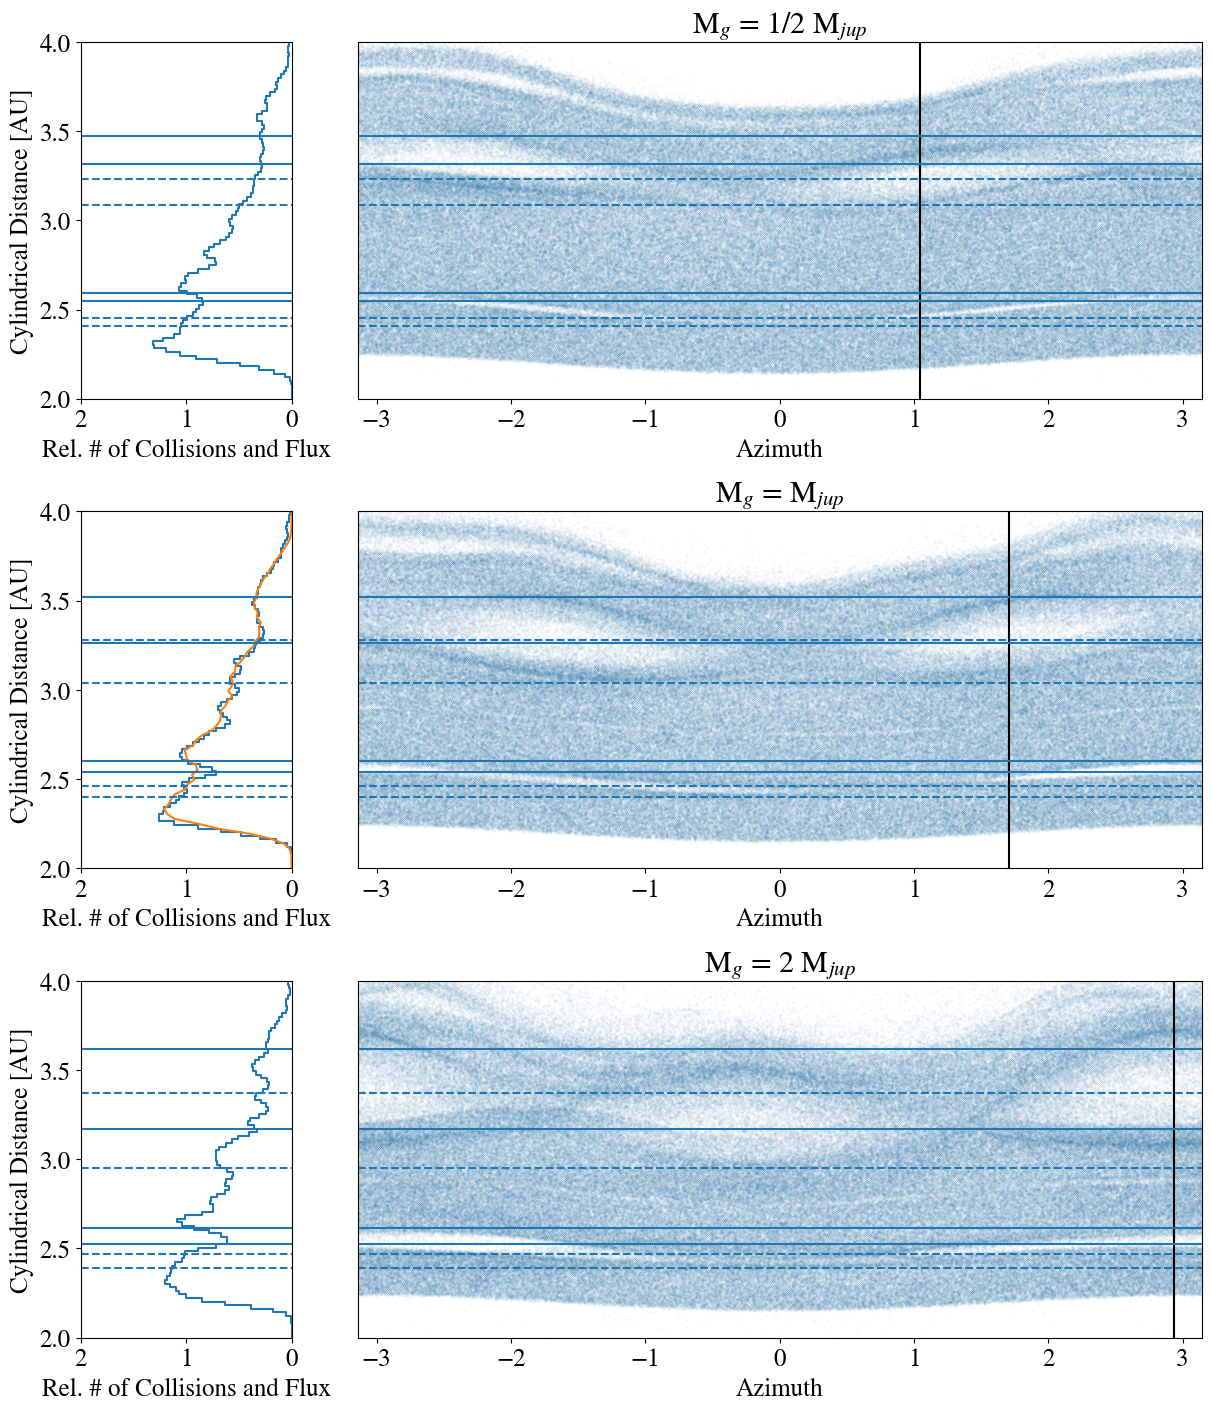
\includegraphics[width=\textwidth]{figures/coll_polar_m.png}
    \caption{Similar to the previous figure, except the eccentricity of the planet is kept constant and the mass is varied.
    This has the effect of changing the width of the resonances, without altering the relative apo or peri distances of
    bodies near the edges.\label{fig:coll_polar_m}}
\end{figure*}

\begin{figure*}
\begin{center}
    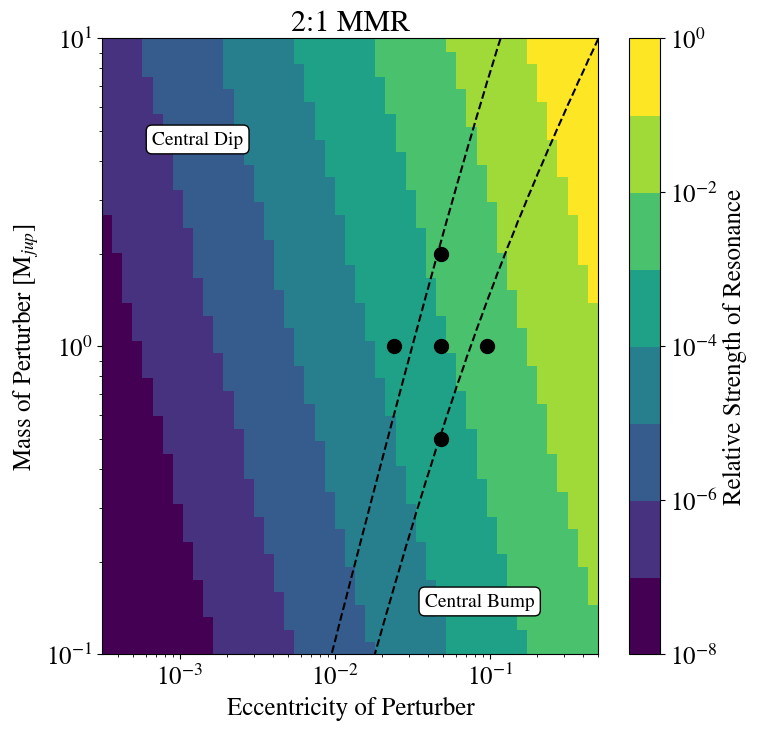
\includegraphics[width=\textwidth]{figures/bump_dip_diag.png}
    \caption{The presence of a dip or bump near the resonances can be used to constrain the mass and eccentricity
    of the perturbing planet. The color scale indicates the relative strength of the features, while the dashed lines
    indicate boundaries in parameter space where a dip or a bump will be produced at the resonance.\label{fig:bump_dip_diag}}
\end{center}
\end{figure*}

\subsection{Collision Rates}\label{sec:coll_rates}

\subsection{Where Does the Dust End Up?}

\section{Influence of Jupiter's Mass and Eccentricity on the Radial Dust Profile}

\section{Observability of Dust} \label{sec:dust}

Aaron's CASA images go here

\section{Summary and Discussion} \label{sec:discuss}

\bibliography{references}

\clearpage

\end{document}
